\section*{Learning Objectives}

\begin{itemize}
\item Begin to understand the vocabulary of mathematics and programming
\item Answer the question: why make a distinction between integers and decimal numbers.
\item An introduction to the most important tools of linear algebra: vectors and matrices.
\item Find out an easy way to determine when a set of linear equations has a unique answer.
\end{itemize}

\section*{Outcomes}
\begin{itemize}
    \item Scalars vs Array
    \item Row vectors and column vectors
    \item Rectangular matrices and square matrices
    \item Learn new mathematical notation $x:=y$, which means that $x$ is by definition equal to $y$. You may be more used to $x \triangleq y$. 
    \item Using matrices and vectors to express systems of linear equations
    \item Determinant of a square matrix and its relation to uniqueness of solutions of systems of linear equations
    \end{itemize}
    
\newpage

\section{Scalars and Arrays}

\textit{Scalars} are simply numbers such as the ones you have been using for a long time: 25.77763, $\sqrt{17}, 10, -4, \pi$. In the Julia programming language, you will soon learn that for computational and storage efficiency, Julia differentiates between scalars that require decimal points and those that do not. Get ready for that! In ROB 101, when we do math, scalars are just numbers. When we do programming, scalars that do not require decimal points are called INTEGERS and those that do require decimal points are called FLOATING POINT NUMBERS because, with the same number of zeros and ones\footnote{Zeros and ones are sometimes called the binary language of computers. If you are interested in binary numbers and binary arithmetic, you can find many sources on the web.}, Julia has to represent very large numbers such as $5.972 \times 10^{24}$, the mass of the earth in kilograms, and very small numbers, such as the mass of one atom of lead in kilograms $3.4406366 \times 10^{-22}$. To do that, where the decimal point appears in a list of zeros and ones has to ``float'', that is, it varies from number to number.\\


In ROB 101, we will not need to learn how computers represent numbers in \textit{binary}. We will simply accept that computers use a different representation for numbers than we humans use. The more zeros and ones we allow in the representation of number, the more space it takes and the longer it takes to add them or multiply them, etc. The \href{https://en.wikipedia.org/wiki/Apollo_Guidance_Computer}{computer} that  provided navigational assistance for the moon landing on 20 July 1969 had a 16 bit word length, meaning its computations were based on groups of 16 binary digits (zeros and ones), called \textit{bits}. In Julia, we'll typically use 64 zeros and ones to represent numbers: 
\begin{itemize}
    \item Int64
    \item Float64
\end{itemize}

\textbf{Remark (can skip)}: In case you are wondering, $\infty$ (infinity) is a concept: it is NOT a number. Because it is not a number, $\infty$ is neither an integer nor a decimal number. The symbol $\infty$ is used to indicate that there is no positive upper bound for how big something can grow (i.e., it can get bigger and bigger and bigger $\ldots$), while $-\infty$ is similar to indicate that something can get more and more negative without end. In ROB 101, you will only encounter $\infty$ when you try to divide something by zero. Julia has been programmed to rock your world when you do that! (Just kidding).

\vspace*{1cm}

    \begin{figure}[h!]
\centering
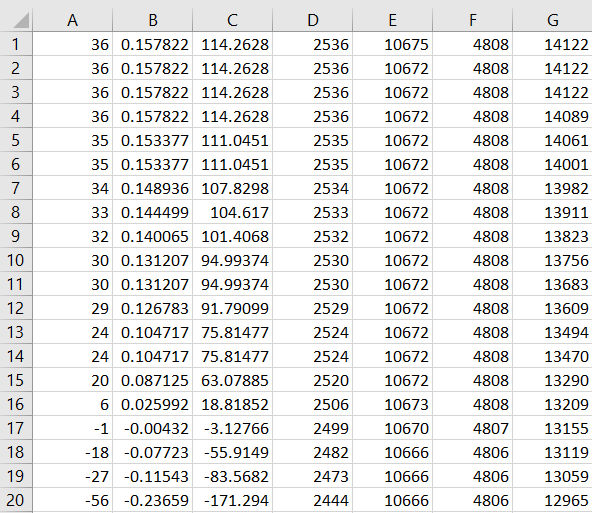
\includegraphics[width=0.6\textwidth]{Chap02_VectorsMatrices/ExcelArray.png}
\caption{Here is an array of numbers from a spreadsheet. The rows are numbered while the columns are labeled with letters. }
    \label{fig:Chapt2:spreasheet}
\end{figure}
\newpage

\textit{Arrays} are scalars that have been organized somehow into lists. The lists could be rectangular or not, they could be made of columns of numbers, or rows of numbers. If you've ever used a spreadsheet, then you have seen an array of numbers. In Fig.~\ref{fig:Chapt2:spreasheet}, columns A, D, E, F, and G have only integer numbers in the them, while columns B and C use decimal numbers. Each row has both integer numbers and decimal numbers.


\section{Row Vectors and Column Vectors}

For us, a \textit{vector} is a finite ordered list of numbers or of unknowns. In Julia, a vector is a special case of an \textit{array}. For example 
\begin{equation}
    \label{eq:firstColumnVector}
    v=\left[\begin{array}{r} 1.1 \\ -3~~~ \\ 44.7 \end{array} \right]
\end{equation}
is a vector of \textit{length} three; sometimes we may call it a \textit{3-vector}. By \textit{ordered} we mean the list has a first element $v_1=1.1$, a second element $v_2=-3$, and a third element $v_3=44.7$, and we also mean that if we change the order in which we list the elements, we (usually) obtain a different vector. For example, the vector 
\begin{equation}
    \label{eq:secondColumnVector}
    w=\left[\begin{array}{r} 1.1 \\  44.7 \\ -3~~~  \end{array} \right]
\end{equation}
is not equal to the vector $v$, even though they are made of the same set of three numbers. \\

Vectors written from ``top'' to ``bottom'' as in \eqref{eq:firstColumnVector} and \eqref{eq:secondColumnVector} are called \textit{column} vectors. It is also useful to write vectors from ``left'' to ``right'' as in 
\begin{equation}
    \label{eq:firstRowVector}
    v^{\rm row}=\left[\begin{array}{ccc} 1.1 & -3 & 44.7 \end{array} \right]
\end{equation}
and we call them \textit{row} vectors. What we said about the word ``ordered'' applies equally well to row vectors in that the row vector $v$ has a first element $v_1^{\rm row}=1.1$, a second element $v_2^{\rm row}=-3.0$, and a third element $v_3^{\rm row}=44.7$. Moreover, if we change the order in which we list the elements, we (usually) obtain a different row vector. Here, we were super careful and added the superscript $^{\rm row}$ to $v^{\rm row}$ to clearly distinguish the symbol $v$ being used for the column vector \eqref{eq:firstColumnVector} from the row vector \eqref{eq:firstRowVector}. Normally, we will not be that fussy with the notation, BUT, you must be aware that column vectors and row vectors are different ``animals'' except in the case that they have length one, as in $v=[v_1]$ is both a row vector and a column vector.\\

A general length $n$ column vector is written like this,
\begin{equation}
    \label{eq:nColumnVector}
    v=\left[\begin{array}{c} v_1 \\ \vdots \\ v_n \end{array} \right],
\end{equation}
while a general length $n$ row vector is written like this
\begin{equation}
    \label{eq:nRowVector}
    v=\left[\begin{array}{ccc} v_1 & \cdots & v_n \end{array} \right].
\end{equation}
This general notation allows for the case that $n=1$, yielding
$$v=[v_1], $$
which as we noted above, is both a row vector and a column vector. \\

Here are some examples in Julia, thanks to Prof. Maani Ghaffari:
\begin{lstlisting}[language=Julia,style=mystyle]
# we define an array of numbers.
# a is a 1x5 array
a = [1 -2 4 8.1 2^0.5]
\end{lstlisting}
\textbf{Output}
\begin{verbatim}
1×5 Matrix{Float64}:
 1.0  -2.0  4.0  8.1  1.41421
\end{verbatim}

\begin{lstlisting}[language=Julia,style=mystyle]
# b is a 5x1 array
b = [1, -2, 4, 8.1, 2^0.5]
\end{lstlisting}
\textbf{Output}
\begin{verbatim}
5-element Vector{Float64}:
  1.0
 -2.0
  4.0
  8.1
  1.4142135623730951
\end{verbatim}

\begin{lstlisting}[language=Julia,style=mystyle]
# b is a 5x1 array
b = [1, -2, 4, 8.1, 2^0.5]
\end{lstlisting}
\textbf{Output}
\begin{verbatim}
5-element Vector{Float64}:
  1.0
 -2.0
  4.0
  8.1
  1.4142135623730951
\end{verbatim}
\begin{lstlisting}[language=Julia,style=mystyle]
# or 
c = [1; -2; 4; 8.1; 2^0.5]
\end{lstlisting}
\textbf{Output}
\begin{verbatim}
5-element Vector{Float64}:
  1.0
 -2.0
  4.0
  8.1
  1.4142135623730951
\end{verbatim}

\section{Remark on Brackets}

Usually, in this course and in most books, \textit{square brackets} $[~~]$ are used to enclose vectors, but that is mainly \textit{a matter of taste} as you can also use \textit{parentheses} $(~~)$ as in
\begin{equation}
    \label{eq:nColumnVectorParen}
    v=\left(\begin{array}{c} v_1 \\ \vdots \\ v_n \end{array} \right)
\end{equation}
and 
\begin{equation}
    \label{eq:nRowVectorParen}
    v=\left(\begin{array}{ccc} v_1 & \cdots & v_n \end{array} \right).
\end{equation}
\textbf{In most programming languages, and Julia is no exception, you can only use square brackets!} The choice of symbols, words, and their allowed arrangements in a language is called \textit{syntax}. In a  programming language, syntax is typically much more restrictive than in a written version of a spoken language. At some point, you may appreciate that throwing errors for bad syntax helps us to reduce \textit{ambiguity} and \textit{bugs} when we program. \textit{You have likely experienced that ambiguities in spoken language can sometimes lead to bad outcomes.} 

\section{Matrices, Rectangular and Square, and the Matrix Diagonal}

Matrices are generalizations of vectors that allow multiple columns and rows, where each row must have the same number of elements\footnote{Equivalently, each column has the same number of elements.}. Here is a $3\times 2$ matrix, 
\begin{equation}
 A=\left[\begin{array}{cc} 1 & 2\\
3 & 4 \\ 5 & 6 \end{array}\right],   
\end{equation}
meaning it has three rows and two columns, while here is a $2 \times 3$ matrix,
\begin{equation}
 A=\left[\begin{array}{rrr} 1.2 & -2.6 & 11.7\\
3.1 & \frac{11}{7} & 0.0\end{array}\right],   
\end{equation}
meaning it has two rows and three columns. It is customary to call a $1 \times n$ matrix a row vector and an $n \times 1$ matrix a column vector, but it is perfectly fine to call them matrices too! \\

A general $n \times m$ matrix 
\begin{equation}
\label{eq:rectangularMatrix}
 A=\left[\begin{array}{cccc} a_{11} & a_{12} & \cdots & a_{1m}\\
a_{21} & a_{22} & \cdots & a_{2m} \\ \vdots & \vdots & \ddots& \vdots \\
a_{n1} & a_{n2} & \cdots & a_{nm}\\\end{array}\right],   
\end{equation}
is said to be \textit{rectangular of size $n \times m$} (one reads this as ``$n$ by $m$''), and when $n=m$, we naturally say that the $n \times n$ matrix
\begin{equation}
\label{eq:squareMatrix}
 A=\left[\begin{array}{cccc} a_{11} & a_{12} & \cdots & a_{1n}\\
a_{21} & a_{22} & \cdots & a_{2n} \\ \vdots & \vdots & \ddots& \vdots \\
a_{n1} & a_{n2} & \cdots & a_{nn}\\\end{array}\right] 
\end{equation}
is \textit{square}.
We note that $a_{ij}$, the $ij$-element of $A$, lies on the intersection of the $i$-th row and the $j$-th column. \\

\begin{tcolorbox}
\textbf{Definition:} The \textbf{diagonal} of the square matrix $A$ in \eqref{eq:squareMatrix} is
\begin{equation}
    {\rm diag}(A)=\begin{bmatrix}a_{11} & a_{22} & \ldots & a_{nn} \end{bmatrix}
\end{equation}
What we are calling the diagonal is sometimes called the \textit{main diagonal of a matrix}. We now highlight the diagonal in red to help those with a ``visual memory''
$$
 A=\left[\begin{array}{cccc} \RED a_{11} & a_{12} & \cdots & a_{1n}\\
a_{21} & \RED a_{22} & \cdots & a_{2n} \\ \vdots & \vdots & \RED \ddots& \vdots \\
a_{n1} & a_{n2} & \cdots & \RED a_{nn}\\\end{array}\right] \iff {\rm diag}(A)=\begin{bmatrix}\RED a_{11} & \RED a_{22} & \RED \ldots & \RED a_{nn} \end{bmatrix}.
$$
\end{tcolorbox}

While it is possible to define the diagonal of general rectangular matrices, we will not do so at this time. Here are some examples in Julia, once again thanks to Prof. Maani Ghaffari
\begin{lstlisting}[language=Julia,style=mystyle]
# Let's define a 3x2 matrix
A = [1 2; 3 4; 5 6]
\end{lstlisting}
\textbf{Output}
\begin{verbatim}
3×2 Array{Int64,2}:
 1  2
 3  4
 5  6
\end{verbatim}
\begin{lstlisting}[language=Julia,style=mystyle]
# Let's define a 2x3 matrix
A = [1.2 -2.6 11.7; 3.1 11/7 0]
\end{lstlisting}
\textbf{Output}
\begin{verbatim}
2×3 Array{Float64,2}:
 1.2  -2.6      11.7
 3.1   1.57143   0.0
\end{verbatim}
\begin{lstlisting}[language=Julia,style=mystyle]
# Here is a big matrix
using Random
A = randn(6,6)
\end{lstlisting}
\textbf{Output}
\begin{verbatim}
6×6 Matrix{Float64}:
 -0.518479   0.693952  -0.137698    0.200556   2.03276   -1.09174
  0.575811   0.999473  -0.0427593  -0.903915   2.14338    0.240728
  0.570255   0.477523  -0.503201   -0.864054  -0.661544   0.0821051
 -0.681514  -1.02591   -0.418878    0.248959  -0.776872   0.466698
  0.395184   1.72782    0.976437    1.10196    0.892258  -1.48822
  1.15146   -0.161273  -0.691775   -1.07168    0.909486  -1.02277
\end{verbatim}
\begin{lstlisting}[language=Julia,style=mystyle]
# compute its diagonal
using LinearAlgebra
diagA=diag(A)
\end{lstlisting}
\textbf{Output}
\begin{verbatim}
6-element Vector{Float64}:
 -0.5184785168661076
  0.9994728076152639
 -0.5032006177084569
  0.24895902626040853
  0.8922580664116776
 -1.022769405730864
\end{verbatim}

\section{Expressing a System of Linear Equations in terms of Vectors and Matrices}

Before we even talk about ``matrix-vector multiplication'', we can address the task of writing a system of linear equations in ``matrix-vector form''. In the beginning, we will diligently follow the notation $Ax=b$, so let's see how we can identify a matrix $A$, a column vector $x$, and a column vector $b$. We'll do a few examples before giving a ``general method''. 


\begin{example}
\label{ex:ExpressMatrixForm01}
Express the System of Linear Equations in Matrix Form: 
\begin{equation}
\label{eq:Axeqb01}
\begin{aligned}
x_1+x_2 &=4 \\
2x_1-x_2&=-1.
\end{aligned}
\end{equation}

\end{example}

\textbf{Solution:}
When your instructors look at this equation, they see two unknowns $x_1$ and $x_2$ and \textit{coefficients\footnote{Coefficients in this case are the numbers multiplying $x_1$ and $x_2.$ An equations typically has variables (unknowns) and coefficients (numbers) that multiply the unknowns or that determine what the equation is supposed to equal, as in $3x_1 + 4 x_2 =7$.}} associated with them on the left-hand and right-hand sides of the two equations.\\

We can use the unknowns to define a column vector of length two, the four coefficients multiplying the unknowns to build a $2 \times 2$ matrix $A$, and the two coefficients on the right-hand side to define another column vector of length two, 
 \begin{equation}
\label{eq:Axeqb02}
\begin{aligned}
x_1+x_2 &=4 \\
2x_1-x_2&=-1
\end{aligned} \iff \underbrace{\left[\begin{array}{rr} 1 & 1\\
2 & -1 \end{array}\right]}_{A} \underbrace{\left[\begin{array}{c} x_1\\
x_2\end{array}\right]}_{x} =   \underbrace{\left[\begin{array}{r} 4\\
-1\end{array}\right]}_{b}.
\end{equation}
\Qed

\begin{example}
\label{ex:ExpressMatrixForm02}
Express the System of Linear Equations in Matrix Form: 
\begin{equation}
\begin{aligned}
x_1-x_2 &=1 \\
2x_1-2x_2&=-1.
\end{aligned}
\end{equation}

\end{example}

\textbf{Solution:}
We now jump straight into it. We form the $2 \times 1$ vector $x$ of unknowns as before and place the coefficients by rows into the $2 \times 2$ matrix $A$,
\begin{equation}
\label{eq:Axeqb03}
\begin{aligned}
x_1-x_2 &=1 \\
2x_1-2x_2&=-1
\end{aligned} \iff \underbrace{\left[\begin{array}{rr} 1 & -1\\
2 & -2 \end{array}\right]}_{A} \underbrace{\left[\begin{array}{c} x_1\\
x_2\end{array}\right]}_{x} =   \underbrace{\left[\begin{array}{r} 1\\
-1\end{array}\right]}_{b}.
\end{equation}
\Qed

\begin{example}
\label{ex:ExpressMatrixForm02BB}
Express the System of Linear Equations in Matrix Form: 
\begin{equation}
\begin{aligned}
3x_1+x_2+2x_3 &=7 \\
2x_1-x_2+4x_3&=4
\end{aligned}
\end{equation}
\end{example}

\textbf{Solution:} We can have the number of equations different from the number of unknown variables. In this case, we have more unknowns than equations. 
\begin{equation}
\label{eq:Axeqb04D}
\begin{aligned}
3x_1+x_2+2x_3 &=7 \\
2x_1-x_2+4x_3&=4
\end{aligned}
\iff \underbrace{\left[\begin{array}{rrr} 3 & 1 & 2\\
2 & -1 & 4\end{array}\right]}_{A} \underbrace{\left[\begin{array}{c} x_1\\ x_2 \\ x_3\end{array}\right]}_{x} =   \underbrace{\left[\begin{array}{c} 7\\ 4 \end{array}\right]}_{b}
\end{equation}
\Qed


\begin{tcolorbox}[sharp corners, colback=green!30, colframe=green!80!blue, title={\bf \Large From Multiple Linear Equations to Matrices and Vectors}]
We will work an example with three equations and four variables. The same method works for $n$ equations in $m$ variables. \textbf{Goal:} Transform a system of linear equations into matrix form $Ax = b$
\begin{equation}
\label{eq:3Eqns4unknowns}
\begin{aligned}
a_{11} x_1+ a_{12}x_2 + a_{13}x_3 + a_{14}x_4&=b_1 \\
a_{21} x_1+ a_{22}x_2 + a_{23}x_3 + a_{24}x_4&=b_2 \\
a_{31} x_1+ a_{32}x_2 + a_{33}x_3 + a_{34}x_4&=b_3.
\end{aligned}
\end{equation}

Two parts are really easy. We define two column vectors
\begin{equation}
    \label{eq:DefinexDefineb}
    x :=\begin{bmatrix} x_1 \\ x_2 \\x_3 \\x_4\end{bmatrix}\text{ and }  b :=\begin{bmatrix} b_1 \\ b_2 \\b_3 \end{bmatrix}.
\end{equation}
The vector $x$ has four rows because there are $m=4$ unknowns, $x_1, x_2, x_3$ and $x_4$. The vector $b$ has three rows because there are $n=3$ equations.\\

Now, what about the matrix $A$? First of all, it's size is $3 \times 4$ because it has one row for each equation and one column for each unknown. You can think about it as follows. We place each term $a_{ij} x_j$ in the entry corresponding to the $i$-th row and $j$-th column. For example $a_{23}x_3$ goes in the second row and third column; we highlight it below
\begin{equation}
\label{eq:3Eqns4unknowns_part02}
 \begin{array}{c}  row_1 \\ row_2\\row_3 \end{array}  \underbrace{ \left[ \begin{array}{cccc}
a_{11} x_1& a_{12}x_2 &  a_{13}x_3 & a_{14}x_4 \\
a_{21} x_1& a_{22}x_2 &  \RED a_{23}x_3 & a_{24}x_4 \\
a_{31} x_1& a_{32}x_2 & a_{33}x_3 & a_{34}x_4
\end{array} \right] }_{\begin{array}{cccc} col_1~~ & ~~~~col_2~~& ~~~col_3 & ~~col_4 ~~\end{array}}  = \begin{bmatrix} b_1 \\ b_2 \\b_3 \end{bmatrix}.
\end{equation}
We note that $row_1$ of the matrix has the terms for the first equation, $row_2$ has the terms for the second equation, etc, while $col_1$ is for the $x_1$ terms of each of the equations,  $col_2$ is for the $x_2$ terms, etc. If we add up all of the entries in a given row, we obtain the corresponding equation.\\

Next, we move the $x_i$'s out of the matrix to the right-hand side while leaving the coefficients where they are, like so
\begin{equation}
\label{eq:3Eqns4unknowns_part03}
  \begin{array}{c}  row_1 \\ row_2\\row_3 \end{array}  \underbrace{ \left[ \begin{array}{cccc}
a_{11} x_1& a_{12}x_2 &  a_{13}x_3 & a_{14}x_4 \\
a_{21} x_1& a_{22}x_2 &  \RED a_{23}x_3 & a_{24}x_4 \\
a_{31} x_1& a_{32}x_2 & a_{33}x_3 & a_{34}x_4
\end{array} \right] }_{\begin{array}{cccc} col_1~~ & ~~~~col_2~~& ~~~col_3 & ~~col_4 ~~\end{array}}  = \begin{bmatrix} b_1 \\ b_2 \\b_3 \end{bmatrix} \iff \begin{array}{c}  Eq_1 \\ Eq_2\\ Eq_3 \end{array}  \underbrace{  \left[ \begin{array}{cccc}
a_{11} & a_{12} &  a_{13} & a_{14} \\
a_{21} & a_{22} &  \RED a_{23} & a_{24} \\
a_{31}& a_{32}& a_{33} & a_{34}
\end{array} \right] }_{\begin{array}{cccc} ~~~~var_1 & var_2& var_3 & var_4 ~~\end{array}} \begin{bmatrix}x_1 \\x_2 \\ x_3 \\ x_4 \end{bmatrix} = \begin{bmatrix} b_1 \\ b_2 \\b_3 \end{bmatrix}
\end{equation}
to obtain 
\begin{equation}
\label{eq:equiavelentLinearEquations}
\begin{aligned}
a_{11} x_1+ a_{12}x_2 + a_{13}x_3 + a_{14}x_4&=b_1 \\
a_{21} x_1+ a_{22}x_2 + a_{23}x_3 + a_{24}x_4&=b_2 \\
a_{31} x_1+ a_{32}x_2 + a_{33}x_3 + a_{34}x_4&=b_3.
\end{aligned} \iff 
\underbrace{  \left[ \begin{array}{cccc}
a_{11} & a_{12} &  a_{13} & a_{14} \\
a_{21} & a_{22} &   a_{23} & a_{24} \\
a_{31}& a_{32}& a_{33} & a_{34}
\end{array} \right] }_{A} \underbrace{\begin{bmatrix}x_1 \\x_2 \\ x_3 \\ x_4 \end{bmatrix}}_{x} = \underbrace{\begin{bmatrix} b_1 \\ b_2 \\b_3 \end{bmatrix}}_{b}
\end{equation}

\textbf{Remark:} After a bit of practice, you will go straight from \eqref{eq:3Eqns4unknowns} to \eqref{eq:3Eqns4unknowns_part03} (in other words, from the left-hand side of \eqref{eq:equiavelentLinearEquations} to the right-hand side of \eqref{eq:equiavelentLinearEquations}), without passing through the intermediate step given in  \eqref{eq:3Eqns4unknowns_part02}. 

\end{tcolorbox}

\begin{example}
\label{ex:ExpressMatrixForm03}
Express the System of Linear Equations in Matrix Form: 
\begin{equation}
\begin{aligned}
x_1+x_2+2x_3 &=7 \\
2x_1-x_2+x_3&=0.5\\
x_1 + 4 x_3 &=7
\end{aligned}
\end{equation}
\end{example}

\textbf{Solution:} Note that we treat ``any missing coefficients'' (as in the ``missing $x_2$'' in the third equation) as being zeros! This is super important to remember. 
\begin{equation}
\label{eq:Axeqb04}
\begin{aligned}
x_1+x_2+2x_3 &=7 \\
2x_1-x_2+x_3&=0.5\\
x_1 + 4 x_3 &=7
\end{aligned}
\iff \underbrace{\left[\begin{array}{rrr} 1 & 1 & 2\\
2 & -1 & 1 \\ 1 & \boxed{0} & 4\end{array}\right]}_{A} \underbrace{\left[\begin{array}{c} x_1\\ x_2 \\ x_3\end{array}\right]}_{x} =   \underbrace{\left[\begin{array}{c} 7\\ 0.5 \\ 7\end{array}\right]}_{b}
\end{equation}
\Qed

\begin{example}
\label{ex:ExpressMatrixForm03B}
We redo Example~\ref{ex:ExpressMatrixForm03}  with the equations in a different order
\begin{equation}
\begin{aligned}
x_1 + 4 x_3 &=7 \\
x_1+x_2+2x_3 &=7 \\
2x_1-x_2+x_3&=0.5
\end{aligned}
\end{equation}
\end{example}

\textbf{Solution:} Once again,  we treat ``any missing coefficients'' (as in the ``missing $x_2$'' in the first equation) as being zeros! This is super important to remember. 
\begin{equation}
\label{eq:Axeqb04C}
\begin{aligned}
x_1 + \boxed{ 0 x_2} +  4 x_3 &=7\\
x_1+x_2+2x_3 &=7 \\
2x_1-x_2+x_3&=0.5\\
\end{aligned}
\iff \underbrace{\left[\begin{array}{rrr} 1 & \boxed{0} & 4 \\ 1 & 1 & 2\\
2 & -1 & 1 \end{array}\right]}_{A} \underbrace{\left[\begin{array}{c} x_1\\ x_2 \\ x_3\end{array}\right]}_{x} =   \underbrace{\left[\begin{array}{c} 7 \\ 7\\ 0.5\end{array}\right]}_{b}
\end{equation}
\Qed

\begin{example}
\label{ex:ExpressMatrixForm03C}
(Optional Read) We redo Example \ref{ex:ExpressMatrixForm03}  \textcolor{red}{with the equations {\bf and variables}} in a different order
\begin{equation}
\begin{aligned}
x_1+x_2+2x_3 &=7 \\
x_1 + 4 x_3 &=7 \\
2x_1-x_2+x_3&=0.5
\end{aligned}
\end{equation}
\end{example}

\textbf{Solution:} This time, just to drive home the point that you can place the variables in any order that you wish, we will define $x$ by
$$ x_{\rm odd} = \left[\begin{array}{c} x_2\\ x_3 \\ x_1\end{array}\right]. $$
With the variables $x_1$, $x_2$, and $x_3$ arranged in this deliberately strange order, the matrices become
\begin{equation}
\label{eq:Axeqb04C2}
\begin{aligned}
x_1+x_2+2x_3 &=7 \\
x_1 + \boxed{ 0 x_2} +  4 x_3 &=7\\
2x_1-x_2+x_3&=0.5\\
\end{aligned}
\iff \underbrace{\left[\begin{array}{rrr}  1 & 2 & 1 \\ \boxed{0} & 4 & 1  \\
 -1 & 1 & 2 \end{array}\right]}_{A_{\rm odd}} \underbrace{\left[\begin{array}{c} x_2\\ x_3 \\ x_1\end{array}\right]}_{x_{\rm odd}} =   \underbrace{\left[\begin{array}{c} 7 \\  7 \\0.5 \end{array}\right]}_{b}
\end{equation}
\textcolor{blue}{\bf Re-ordering the components of $x$ re-orders the columns of $A$.} 
\Qed

\vspace*{0.2cm}

\begin{tcolorbox}[sharp corners, colback=green!30, colframe=green!80!blue,title=\textbf{How to Handle ``Missing'' Variables or Coefficients}]
A zero in row $i$ and column $j$ of a matrix corresponds to the variable $x_j$ being absent from the $i$-th equation
\begin{equation}
\label{eq:Axeqb05}
\underbrace{\left[\begin{array}{rrr} 0 & 0 & 2\\
2 & 0 & 0 \\ 
0& -1 & 4\end{array}\right]}_{A} 
\underbrace{\left[\begin{array}{c} x_1\\ x_2 \\ x_3\end{array}\right]}_{x} =   \underbrace{\left[\begin{array}{c} 7\\ 0.5 \\ 7\end{array}\right]}_{b} \iff \begin{aligned}
2x_3 &=7 \\
2x_1&=0.5\\
-x_2 + 4 x_3 &=7
\end{aligned} \iff \underbrace{\begin{aligned}
0x_1 + 0 x_2 + 2x_3 &=7 \\
2x_1 + 0 x_2 + 0 x_3&=0.5\\
0 x_1 -x_2 + 4 x_3 &=7
\end{aligned}}_{\text{we'd never write it like this}} 
\end{equation}
\end{tcolorbox}


\section{The Matrix Determinant}

One of the more difficult topics in \textit{Linear Algebra} is the notion of the determinant of a matrix. Most people who claim to understand it are wrong. Instead of teaching you right away a bunch of details of the matrix determinant that are rather useless in the actual practice of Linear Algebra, we are going to cut directly to the ``good stuff''. Moreover, we'll only give you part of the good stuff here, and save some ``really excellent stuff'' for Chapter \ref{chap:MatrixProductInversesDeterminants}. 


\subsection{First Contact with the Matrix Determinant}
\label{sec:OperationalDeterminant}

% \begin{tcolorbox}%%[]


% \end{tcolorbox}

What you want and need to know about the determinant function: the first five points are extra important.

\begin{tcolorbox}[sharp corners, colback=green!30, colframe=green!80!blue, title=\textbf{Enough Facts about the Determinant to Get Us Going}]
\begin{enumerate}[label={Fact~}{\arabic*}]

\item \label{item:determinantFact0}  The determinant of a square matrix $A$ is a real number, denoted $\det(A)$.

    \item \label{item:determinantFact1} A square system of linear equations (i.e.,  $n$ equations and $n$ unknowns), 
    $Ax=b,$
    has a unique solution $x$ for any $n\times 1$ vector $b$ if, and only if, $\det(A) \neq 0.$
    
     \item When $\det(A)=0$, the set of linear equations $Ax=b$ may have either no solution or an infinite number of solutions. To determine which case applies (and to be clear, only one case can apply), depends on how ``$b$ is related to $A$'', which is another way of saying that we will have to address this later in the course. 
     
     \item The determinant of the $1 \times 1$ matrix $A=[a]$ is $\det(A):=a$.
     
    \item The determinant of the $2 \times 2$ square matrix 
    $A=\left[\begin{array}{cc} a & b \\ c & d \end{array} \right]$ is
  $\det(A):= a d - bc.$
 
     \item The determinant is only defined for square matrices; see~ \ref{item:determinantFact0}.
     
       \item We will learn later how to compute by hand the determinant of $n \times n$ matrices with special structure, but for general matrices, you only need to know how to \textit{compute by hand the determinant of} a $2 \times 2$ matrix.
 
\end{enumerate}

\end{tcolorbox}



\vspace*{.2cm}

\textbf{Remark:} In case you are ``sad'' that  you can only compute determinants for $2\times 2$ matrices, do not worry. \textit{Very soon, you will also be able to do it for a $100 \times 100$ matrix and understand what you are doing.} In this book, we take a ``structural approach'' to Computational Linear Algebra in general, and to the matrix determinant in particular. In Chap.~\ref{chap:Chap03TriangularForwardBAckSubstitution}, we will first focus on matrices with a special ``triangular'' structure and then we'll see how to ``factor'' or ``decompose'' a non-triangular matrix into (the product of) two triangular matrices. This structural approach has many advantages when it comes to scaling up computations to problems with hundreds or even thousands of variables. In particular, it will provide a practical way of understanding and computing the matrix determinant for really big matrices.\\

\textbf{Remark:} A ``clear but advanced'' derivation of the classical formula for the determinant of an $n \times n$ matrix can be found in a blog post by Akihiro Matsukawa: \url{https://mtskw.com/posts/determinant/}. In case the blog post gets taken down, here is a link to a PDF \url{https://tinyurl.com/5n7pm4x} of it. 

\subsection{Examples of Using the Determinant}

We reuse some previous examples and add in a few more to illustrate \ref{item:determinantFact1} of Sec.~\ref{sec:OperationalDeterminant}

\begin{example}
\label{ex:Det01}
Check for existence and uniqueness of solutions:
\begin{equation}
\label{eq:det01b}
\begin{aligned}
x_1+x_2 &=4 \\
2x_1-x_2&=-1
\end{aligned} \iff \underbrace{\left[\begin{array}{rr} 1 & 1\\
2 & -1 \end{array}\right]}_{A} \underbrace{\left[\begin{array}{c} x_1\\
x_2\end{array}\right]}_{x} =   \underbrace{\left[\begin{array}{r} 4\\
-1\end{array}\right]}_{b}.
\end{equation}
\end{example}

\textbf{Solution:}
We compute $\det(A) = (1)\cdot(-1)-(1)\cdot(2) = -3 \neq 0$ and conclude that \eqref{eq:det01b} has a unique solution.
\Qed\\
 


\begin{example}
\label{ex:Det02} 
Check for existence and uniqueness of solutions:
\begin{equation}
\label{eq:det02b}
\begin{aligned}
x_1-x_2 &=1 \\
2x_1-2x_2&=-1
\end{aligned} \iff \underbrace{\left[\begin{array}{rr} 1 & -1\\
2 & -2 \end{array}\right]}_{A} \underbrace{\left[\begin{array}{c} x_1\\
x_2\end{array}\right]}_{x} =   \underbrace{\left[\begin{array}{r} 1\\
-1\end{array}\right]}_{b}
\end{equation}
\end{example}

\textbf{Solution:}
We compute $\det(A) = (1)\cdot(-2)-(-1)\cdot(2) = 0$. We therefore conclude that \eqref{eq:det02b} does not have a unique solution. In fact, it may have either no solution at all or it may have an infinite number of solutions. At this point in the course, we do not have the tools to determine which case applies here without grinding through the equations. Referring back to \eqref{eq:SLE:Ex2}, where we did grind through the equations, we know that this system of linear equations has no solution.
\Qed

\begin{example}
\label{ex:Det03} 
Check for existence and uniqueness of solutions:
\begin{equation}
\label{eq:det03b}
\begin{aligned}
x_1-x_2 &=1 \\
2x_1-2x_2&=2
\end{aligned} \iff \underbrace{\left[\begin{array}{rr} 1 & -1\\
2 & -2 \end{array}\right]}_{A} \underbrace{\left[\begin{array}{c} x_1\\
x_2\end{array}\right]}_{x} =   \underbrace{\left[\begin{array}{r} 1\\
2\end{array}\right]}_{b}
\end{equation}


\end{example}

\textbf{Solution:} We compute $\det(A) = (1)\cdot(-2)-(1)\cdot(2) = 0$. We therefore conclude that \eqref{eq:det03b} does not have a unique solution. In fact, it may have either no solution at all or it may have an infinite number of solutions. At this point in the course, we do not have the tools to determine which case applies here without grinding through the equations. Referring back to \eqref{eq:SLE:Ex3}, we know that this system of linear equations has an infinite number of solutions. 
\Qed


\begin{example}
\label{ex:Det04} 
Check for existence and uniqueness of solutions:
\begin{equation}
\label{eq:det04b}
\begin{aligned}
x_1+x_2+2x_3 &=7 \\
2x_1-x_2+x_3&=0.5\\
x_1 + 4 x_3 &=7 
\end{aligned}
\iff \underbrace{\left[\begin{array}{rrr} 1 & 1 & 2\\
2 & -1 & 1 \\ 1 & 0 & 4\end{array}\right]}_{A} \underbrace{\left[\begin{array}{c} x_1\\ x_2 \\ x_3\end{array}\right]}_{x} =   \underbrace{\left[\begin{array}{c} 7\\ 0.5 \\ 7\end{array}\right]}_{b}
\end{equation}
\end{example}

\textbf{Solution:}
Using Julia, we compute $\det(A) = -9 \neq 0$. We therefore conclude that \eqref{eq:det04b} has a unique solution for $x$.
\begin{lstlisting}[language=Julia,style=mystyle]
# using LinearAlgebra
A=[1 1 2; 2 -1 1; 1 0 4]
det(A)
\end{lstlisting}
\textbf{Output}
\begin{verbatim}
-9.0
\end{verbatim}
\Qed


\begin{example}
\label{ex:Det05} 
Check for existence and uniqueness of solutions in an example where the unknowns are not in the ``correct'' order and we have a bunch of ``missing coefficients'':
\begin{equation}
\label{eq:det05b}
\begin{aligned}
x_1+x_2+2x_3 &=7 \\
-x_2+x_3+2x_1&=0.5\\
x_1 + 4 x_3 &=7 \\
x_4+ 2 x_3 - 5x_5-11&= 0 \\
-4x_2 + 12 x_4 &= 0
\end{aligned}
\iff \underbrace{\left[\begin{array}{rrrrr} 1 & 1 & 2 & 0 & 0\\
2 & -1 & 1  & 0 & 0\\ 1 & 0 & 4 & 0 & 0 \\ 0 & 0 & 2 & 1 & -5 \\ 0 & -4 & 0 & 12 & 0\end{array}\right]}_{A} \underbrace{\left[\begin{array}{c} x_1\\ x_2 \\ x_3 \\x_4 \\x_5\end{array}\right]}_{x} =   \underbrace{\left[\begin{array}{c} 7\\ 0.5 \\ 7 \\ 11 \\ 0\end{array}\right]}_{b}
\end{equation}

\end{example}

\textbf{Solution:}
Using Julia, one computes $\det(A) = -540 \neq 0$. We therefore conclude that \eqref{eq:det05b} has a unique solution. Grinding through the equations would have been no fun at all!
\begin{lstlisting}[language=Julia,style=mystyle]
A=[1 1 2 0 0; 2 -1 1 0 0; 1 0 4 0 0; 0 0 2 1 -5; 0 -4 0 12 0]
det(A)
\end{lstlisting}
\textbf{Output}
\begin{verbatim}
-540.0
\end{verbatim}
\Qed



\section{(Optional Read): Other Facts on the Matrix Determinant Covered in ``Standard'' Courses} 

\vspace*{0.2cm}

Here are some other facts that are sometimes useful but are not required in ROB 101.

\begin{itemize}

 \item In written mathematics, but not in programming, you will also encounter the notation $\det(A) = \left| A \right|,$ so that
  $$\left|\begin{array}{cc} a & b \\ c & d  \end{array} \right|:=ad-bc. $$
  

  \item In Julia, once you state that you are using the linear algebra package, that is \texttt{ using LinearAlgebra}, the command is
  {\texttt  det(A)} , if $A$ is already defined, or, for example, {\texttt  det([1 2 3; 4 5 6; 7 8 9])}
 
  \item The determinant of a $3 \times 3$ matrix is 
\begin{equation}
 \label{eq:3by3Determinant}
  \det \left(  \left[\begin{array}{ccc} a & b & c\\ d & e & f \\ g & h & i \end{array} \right] \right):= a \cdot \det \left(\left[\begin{array}{cc} e & f \\ h & i  \end{array} \right] \right) - b \cdot \det \left(\left[\begin{array}{cc}d & f \\ g & i  \end{array} \right] \right) + c \cdot \det \left(\left[\begin{array}{cc} d & e \\ g & h  \end{array} \right] \right).
\end{equation}
In ROB 101, you do not need to use, much less memorize, the formula \eqref{eq:3by3Determinant}.   

 
\end{itemize}
\vspace*{.2cm}
\begin{tcolorbox}[title=\textbf{Optional, and for sure, skip on your first read: Khan Academy} ]
Here are the (Tiny URLs) of two videos by the Khan Academy that provide a ``clasical'' introduction to the matrix determinant. 
  \begin{itemize}
      \item \url{https://tinyurl.com/gqt93l3} works a $3\times 3$ example based on \eqref{eq:3by3Determinant}.
      \item  \url{https://tinyurl.com/zhlwb5v} shows an alternative way to compute the determinant of a $3 \times 3$ matrix.
      \item \textbf{In ROB 101}, you do not need to use either of these methods.
  \end{itemize}
\end{tcolorbox}

\vspace*{.2cm} 
\begin{figure}[t!]
\centering
\subfloat[]{%
    \label{fig:circuit2Loops}%
	\centering
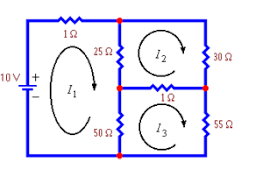
\includegraphics[width=0.4\textwidth]{Chap02_VectorsMatrices/ResistorNetworkLoopMethodKahnAcademy.png}}%
\hspace{5pt}%
\subfloat[]{%
    \label{fig:FitQuadraticEasy}%
	\centering
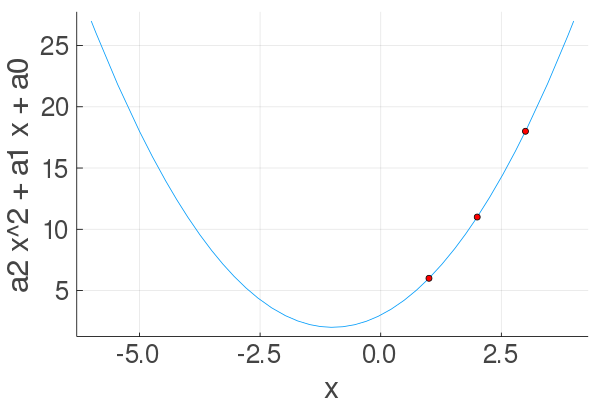
\includegraphics[width=0.42\columnwidth]{Chap02_VectorsMatrices/Quadratic3Points.png}}%
\caption{(a) Image borrowed from the Khan Academy. A simple electric circuit as you would learn to analyze in the first month of EECS 215 using Kirchhoff's Current and Voltage Laws, which can be thought of as the electrical versions of Newton's equations for balancing forces. (b) A quadratic function that you need to find based upon someone having measured for you the three values given in red! Can you do it? Does it matter that the data were selected from only one side of the parabola?}
\label{fig:ResistorNetworkLoopMethodKahnAcademy}
\end{figure}

\section{(Optional Read): A Few ``Practical'' Examples Using Linear Algebra}
You are not responsible for any of these examples. They are given here to provide a sense of how vectors and matrices are used in engineering. Because we are so early in the course, the examples we can work are rather boring and are not on par with what you will do in the projects. 

\begin{example}
\label{ex:CircuitEqualtions}
\textbf{[Circuit Equations]} 
Write the equations satisfied by the currents $I_1$, $I_2$, and $I_3$ in Fig.~\ref{fig:circuit2Loops} and then solve them. 
\end{example}



\textbf{Solution:}
Once you have taken EECS 215, you would quickly write down the following equations which are based on three  facts called Kirchhoff's Current and Voltage Laws:
\begin{itemize}
    \item the sum of the voltages around any loop in the circuit is zero;
    \item current $I$ flowing through resistor $R$ creates a voltage $V = I R$; and 
    \item when two loops touch, as for the 25 $\Omega$ resistor, the currents add with their sign determined by their directions.
\end{itemize}
 At the 25 $\Omega$  resistor, for example, the current is $I_1 - I_2$ because they flow in opposite directions.  In short, after taking EECS 215 and applying Kirchhoff's Current and Voltage Laws, you would obtain
\begin{equation}
\label{eq:circuitb}
\begin{aligned}
-10 + I_1 + 25 (I_1 - I_2) + 50 (I_1 - I_3) &=0 \\
25 (I_2-I_1) + 30 I_2 + (I_2 - I_3)&=0\\
55 I_3 + 50 (I_3 - I_1) + (I_3-I_2) &=0 \\
\end{aligned}
\iff \underbrace{\left[\begin{array}{rrr} 76 & -25 & -50 \\
-25 & 56 & -1  \\ -50 & -1 & 106\end{array}\right]}_{A} \underbrace{\left[\begin{array}{c} I_1\\ I_2 \\ I_3\end{array}\right]}_{x} =   \underbrace{\left[\begin{array}{c} 10\\ 0\\ 0 \end{array}\right]}_{b}
\end{equation}
While it is not important to you, the first equation is obtained by adding up the voltages in the loop with $I_1$, proceeding in the direction of $I_1$, the second equation is obtained by adding up the voltages in the loop with $I_2$, proceeding in the direction of $I_2$, and similarly for the last equation. 
In Julia, we compute that $\det(A)=242,310$, kind of a wild number, but it's non-zero. Solving the equation results in 
$$\left[\begin{array}{c} I_1\\ I_2 \\ I_3\end{array}\right] =  \left[
\begin{array}{c}
0.2449 \\
0.1114 \\
0.1166 \\
\end{array}
\right],$$
in units of Amperes in case you are curious!
\Qed

\begin{example}
\label{ex:FittingEquations}
\textbf{[Fitting a Function to Data]} 
Figure~\ref{fig:FitQuadraticEasy} shows a quadratic function of the form 
\begin{equation}
    \label{eq:quadraticFromData}
    y = a_2 x^2 + a_1 x + a_0.
\end{equation}
You are given the data in Table~\ref{tab:QuadraticDataChap02} and need to find the coefficients $a_2$, $a_1$, and $a_0$ that define the quadratic.
\begin{table}[!hbt]
\caption[]{Data for a Quadratic Function.}
\label{tab:QuadraticDataChap02}
%\spacing 1
\begin{center}
\begin{tabular}{||c|c||}
\hline
 $x$ & $y$\\
\hline
1  &   6 \\
 2    &  11 \\
3   & 18 \\
\hline
\end{tabular}
\end{center}
\end{table}
\end{example}


\textbf{Solution:} Our unknowns are the coefficients $a_2$, $a_1$, and $a_0$. Hence, we rewrite the quadratic as
 $$ y = a_2 x^2 + a_1 x + a_0 = x^2 a_2  + x a_1  + a_0, $$
and note that this equation is linear in the unknowns.
From Table~\ref{tab:QuadraticDataChap02}, we have the following equations
\begin{equation}
\label{eq:qudraticb}
\begin{aligned}
6 &= a_2 + a_1 + a_0 \\
11&= 4 a_2 + 2 a_1 + a_0\\
18&= 9 a_2 + 3 a_1 + a_0\\
\end{aligned}
\iff \underbrace{\left[\begin{array}{rrr} 1 & 1 & 1 \\
4& 2 & 1  \\ 9 & 3 & 1\end{array}\right]}_{A} \underbrace{\left[\begin{array}{c} a_2\\ a_1 \\ a_0\end{array}\right]}_{x} =   \underbrace{\left[\begin{array}{c} 6\\ 11\\ 18 \end{array}\right]}_{b}
\end{equation}
Using Julia, we compute $\det(A)=-2 \neq 0$ and hence a solution to \eqref{eq:qudraticb} exists and is unique. Using our current methods, we compute that the answer is
$$\left[\begin{array}{c} a_2\\ a_1 \\ a_0\end{array}\right] =  \left[
\begin{array}{c}
1.0 \\
2.0\\
3.0 \\
\end{array}
\right].$$
In other words, the data are compatible with the function $y=x^2 + 2 x + 3$. 
\Qed

\vspace*{.2cm}

\begin{example}
\label{ex:FittingEquationsB}
\textbf{[Fitting a Function to Data: Take 2]} We re-visit the quadratic function in 
Fig.~\ref{fig:FitQuadraticEasy} with unknown coefficients $a_2$, $a_1$, and $a_0$, namely
$y = a_2 x^2 + a_1 x + a_0.$ This time, however, we use the data in Table~\ref{tab:QuadraticDataChap02take2}
\begin{table}[!hbt]
\caption[]{Data for a Quadratic Function.}
\label{tab:QuadraticDataChap02take2}
%\spacing 1
\begin{center}
\begin{tabular}{||c|c||}
\hline
 $x$ & $y$\\
\hline
-3 & 6 \\
1  &   6 \\
 2    &  11 \\
3   & 18 \\
\hline
\end{tabular}
\end{center}
\end{table}
\end{example}


\textbf{Solution:} Our unknowns are once again the coefficients $a_2$, $a_1$, and $a_0$. We rewrite the quadratic as
 $$ y = a_2 x^2 + a_1 x + a_0 = x^2 a_2  + x a_1  + a_0, $$
and note again that this equation is linear in the unknowns.
From Table~\ref{tab:QuadraticDataChap02take2}, we have the following equations
\begin{equation}
\label{eq:qudraticc}
\begin{aligned}
6 &= 9 a_2 -3 a_1 + a_0 \\
6 &= a_2 + a_1 + a_0 \\
11&= 4 a_2 + 2 a_1 + a_0\\
18&= 9 a_2 + 3 a_1 + a_0\\
\end{aligned}
\iff \underbrace{\left[\begin{array}{rrr} 9 & -3 & 1 \\ 1 & 1 & 1 \\
4& 2 & 1  \\ 9 & 3 & 1\end{array}\right]}_{A} \underbrace{\left[\begin{array}{c} a_2\\ a_1 \\ a_0\end{array}\right]}_{x} =   \underbrace{\left[\begin{array}{c} 6 \\ 6\\ 11\\ 18 \end{array}\right]}_{b}
\end{equation}
In this case, we have more equations than unknowns, which translates into $A$ being non-square. Because $A$ is non-square, we cannot compute its determinant and then use the answer to determine whether solutions exist or are unique, which is kind of a bummer, because it kind of says that more data is not necessarily better! Later in the course, we will be able to confront this issue head on and learn that, yes, in most cases, more data is better. For now, we punt!
\Qed

\section{(Optional Read)  Yet Another Determinant Example}

In the following examples, the determinant is computed using the method of \eqref{eq:3by3Determinant}. \textbf{You are not required to know this method because you would never want to use it on a $10 \times 10$ matrix, for example,} whereas we will learn a method that scales easily to matrices that are $100 \times 100$. \textcolor{red}{\bf The method in \eqref{eq:3by3Determinant} is only illustrated here to prove a point: it's painful.}\\

\begin{example}
Compute the determinant of the matrix below using the method that is normally taught in Linear Algebra, namely, \eqref{eq:3by3Determinant}.
$$A=\left[\begin{array}{rrr} 4 & -1 & 1\\
4 & 5 & 3 \\ -2 & 0 & 0\end{array}\right] $$

\end{example}

\textbf{Solution:}

\begin{align*}
  \det(A) &= \left|\begin{array}{rrr} 4 & -1 & 1\\
4 & 5 & 3 \\ -2 & 0 & 0\end{array}\right| \\
&= 4 \cdot \left|\begin{array}{rr} 
 5 & 3 \\  0 & 0\end{array}\right| -(-1) \cdot \left|\begin{array}{rr} 
 4 & 3 \\  -2 & 0\end{array}\right| + 1 \cdot  \left|\begin{array}{rr} 
 4 & 5 \\  -2 & 0\end{array}\right| \\
 &\text{ (after applying our determinant formula to each of the 2 x 2 matrices above)}\\
 &= 4 \cdot (0) +1 \cdot(6) + 1\cdot 10\\
 &= 16.
\end{align*}

\Qed


For $3 \times 3$ it's not so bad, but already at $4 \times 4$, it becomes tedious. \\

\begin{example}
Compute the determinant of the matrix below using the method that is normally taught in Linear Algebra.
$$ A=\left[\begin{array}{rrrr} 4 & -1 & 1 & 2\\
4 & 5 & 3 & 7\\ -2 & 0 & 0 & 4\\  -2 & 8 & 1 & 4\end{array}\right] $$
\end{example}

\textbf{Solution:}
\begin{align*}
  \det(A) &= \left|\begin{array}{rrrr} 4 & -1 & 1 & 2\\
4 & 5 & 3 & 7\\ -2 & 0 & 0 & 4\\  -2 & 8 & 1 & 4\end{array}\right| \\
&= 4 \cdot \left|\begin{array}{rrr}
 5 & 3 & 7\\  0 & 0 & 4\\ \  8 & 1 & 4\end{array}\right| - (-1) \left|\begin{array}{rrr} 4 & 3 & 7\\ -2  & 0 & 4\\  -2 & 1 & 4\end{array}\right| + (1)  \left|\begin{array}{rrr} 
4 & 5  & 7\\ -2 & 0 &  4\\  -2 & 8 &  4\end{array}\right| - (2)  \left|\begin{array}{rrr}
4 & 5 & 3 \\ -2 & 0 & 0 \\  -2 & 8 & 1\end{array}\right| \\
& =\text{ (after applying our determinant formula to each of the 3 x 3 matrices above)}\\
& = 4 (76) + 1 (-30) + 1 (-240) - 2 (-38) \\
 &= 110.
\end{align*}
%4* (76) + 1 *(-30) + 1* (-240) - 2* (-38)
\Qed

Once again, the point is not to be understand why this method works or how to do it. The point is how unwieldy it is. Since you have read this far, we'll let you in on a secret. In Chapter~\ref{chap:LUfactorization}, we'll learn how to ``factor'' or ``decompose'' the matrix $A$ above into two matrices called
$$ L =
\left[
\begin{array}{rrrr}
1.0000 & 0.0000 & 0.0000 & 0.0000 \\
-0.5000 & 1.0000 & 0.0000 & 0.0000 \\
1.0000 & 0.8000 & 1.0000 & 0.0000 \\
-0.5000 & -0.0667 & 0.7500 & 1.0000 \\
\end{array}
\right] \text{ and } U=\left[
\begin{array}{rrrc}
4.0 & -1.0 & 1.0 & 2.0 \\
0.0 & 7.5 & 1.5 & 5.0 \\
0.0 & 0.0 & 0.8 & 1.0 \\
0.0 & 0.0 & 0.0 & 55/12 \\
\end{array}
\right].
$$
In Chapter~\ref{chap:MatrixProductInversesDeterminants}, we'll learn that all of the information concerning the determinant is contained in $U$ and that $\det(A) = \det(U) = 4 \times 7.5 \times 0.8 \times 55/12 = 110.0$, the product of the terms on the diagonal of $U$. How mind blowing is that?

\section{Looking Ahead}

We want to solve very large sets of linear equations, say more than 100 variables. We could teach you the matrix inverse command in Julia, but then you'd understand nothing. In the next chapter, we will begin exploring how to solve problems with special structure. Soon after that, we'll show how to transform all linear systems of $n$-equations in $n$-variables to a form where they are solvable with ``special strucutre''. To get there we need to understand:
\begin{itemize}
\item what are \textit{square and triangular matrices};
    \item what is \textit{forward} and \textit{back substitution}; 
     \item what does it mean to multiply two matrices; and
    \item how to \textit{factor} a square matrix as the product of two triangular matrices.
\end{itemize}

 \vspace*{.5cm}
\begin{tcolorbox}[title={\large \textcolor{red}{\bf  Help! Help! } \textbf{ How am I supposed to remember all of this?}}]
 
\textbf{ You probably can't. In any case, we don't want you to memorize the ROB 101 material.} Instead, open up a \texttt{google doc or google sheet} and make notes! You need an organized method for keeping track of stuff. In High School, you may have been able to remember all the new notation without any special effort. In College, it's a bit different.
 
 \end{tcolorbox}

% \section{Some Vector and Matrix Algebra}
% % By now, you probably have absorbed the intuitive idea that two vectors are the ``same'' if the have the same number of elements, listed in the same order. 